% !TEX root = ../thesis.tex

\chapter{案例分析}
流行的数据处理框架比如Hadoop,Spark,Naiad或Hyracks都由托管式语言开发,例如Java,c\#,或Scala。JVM提供的内存自动管理——垃圾收集器(GC)为开发者提供便利。然而,垃圾收集开销是非常大的,GC在这些大数据系统中,可占据高达50\%的执行时间,严重损害了系统的性能。

GC执行缓慢的一个关键原因是大数据系统中的对象特征不匹配传统GC设计使用的启发式算法。在这一章,我们分析一个针对大数据系统中对象行为不匹配的解决方案——Yak。Yak能够智能地适应大数据系统的特性,因此,可以有效地管理在这些大数据系统中存在的大量对象。

我们首先在3.1节介绍Yak的研究思路,然后在3.2节分析该系统的局限性。


\section{研究思路}
\subsection{数据特征不匹配}

传统的分代GC都是基于“已存在时间越短的对象越容易被回收”的假设进行设计的。该假设适用于产生大量短暂临时数据的应用程序,对于这些应用来说, 传统分代GC是有效的——GC扫描一小部分堆就能够回收足够多的内存。但是,大数据应用程序的数据特征与传统分代GC假设不同,这种特征可以概括为两条路径,两种假设。

一个典型的大数据处理框架通常存在控制路径和数据路径的明显区别。控制路径有复杂的执行逻辑(例如,管理和调度集群,建立master node和worker node之间的通信);数据路径主要包括可以连接到一个数据处理管道的数据操作功能(例如,数据分区、Join或Aggregate,用户定义数据功能,例如Map或Reduce)。

这两条路径遵循不同的对象生命特征:控制路径上的对象数量小,存活时间短,生命周期符合分代特征,对它们使用传统的分代GC是合理的;而在数据路径上的对象,它们的生命周期呈现出完全不同的时域(epoch)特征(时域特征指的是一组对象在同一时间被创建,在经历一段较长的程序执行时间后才被同时回收的特征),所以不适合采用传统GC。
\begin{figure}[h]
    \centering
    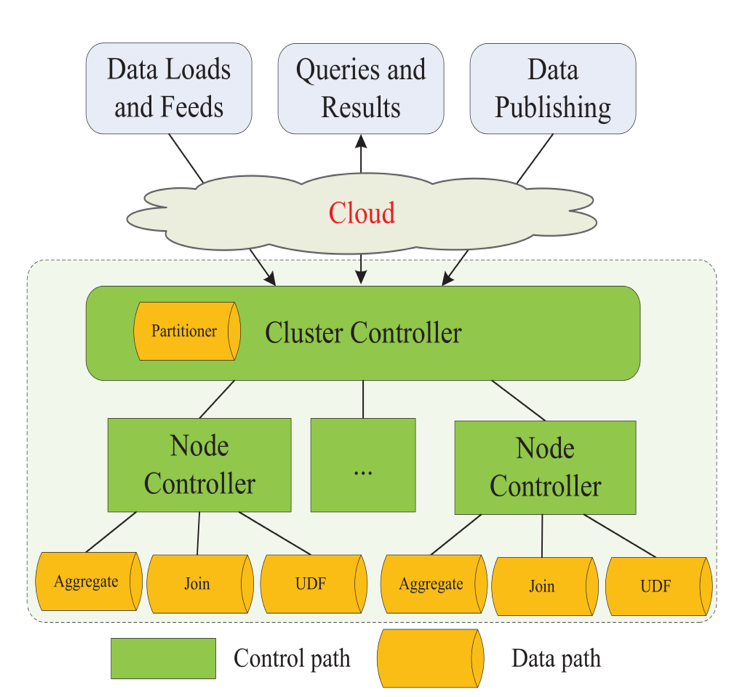
\includegraphics[width=10cm,height=5cm]{figure/two_Path.png}
    \caption{大数据项目架构说明}
\end{figure}

这种不匹配会导致传统分代GC在数据密集型应用程序中的性能瓶颈。因为创建的对象寿命较长,GC的大部分精力都花费在跟踪巨大数量的对象,而不能及时回收内存。 

两条路径,两种特征启发了一种混合内存管理器——用两种不同的方式管理两种路径对象。对于具有时域特征的数据对象提出更加合适的内存管理方式,同一个时域创建的对象分配在同一个内存区域,同时进行内存回收。

\subsection{设计与实现}
\begin{figure}[h]
    \centering
    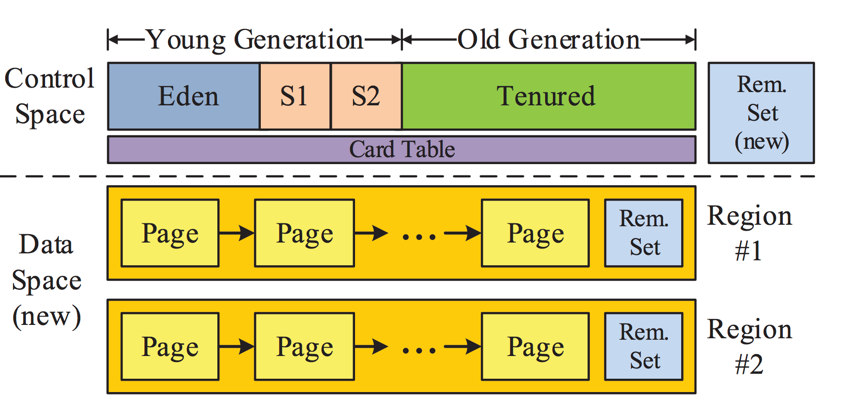
\includegraphics[width=12cm,height=7cm]{figure/layout.png}
    \caption{
        region的一个例子:(a)一个简单的程序被多个线程执行的过程,(b)对应产生的内存域结构
    }
    \label{img3}
\end{figure}
Yak的高层想法是基于明确区分的控制路径和数据路径,把堆分成一个小的控制空间(CS)和一个更大的数据空间(DS), 并使用不同的机制来管理这些空间。控制空间又被划分为新生代、老生代,采用传统的分代内存管理方法;数据空间则由多个内存域(region)组成,采用基于内存域的内存管理方法。
Yak提出以下两个主要设计问题以及解决方案,如图\ref{img3}。

{\bfseries 问题1:何时创建和释放内存域?}

一个时域代表着一段程序的执行。当一个时域开始时,一个内存域被创建;当一个时域结束时,一个内存域被回收。一个内存域储存对应时域创建的所有对象。一个时域可以是用户自定义的,通过注释的方式实现。举例来说,在Hadoop中,一个用户定义的Map任务被setup()和cleanup()两个接口调用建立和关闭,开发者可以对这个两个调用的代码进行注释,从而定义一个时域。

为了建立统一的注释,Yak提供了一对用户注释,epoch\_tart() 和epoch\_end(),这两个注释在运行时被转换成两个本地函数调用,来提醒JVM一个时域的开始和结束。标注这些注释需要的手动工作开销是很小的。即使是新手,没有太多的系统知识,也可以很容易地找到并注释时域。Yak保证执行正确性,当然,时域标注的位置会影响性能:如果一个时域内的对象有不同的寿命,那这些对象会在时域结束后被复制,增加开销。

通常情况下,大数据框架中的系统调用已经具备了很好的时域特性,一旦创建了托管堆(在JVM的启动时期),会保留一系列虚拟地址作为DS。每个时域对应一个内存域,由一组固定长度的内存页组成。

在实践中,需要考虑关于时域概念的更多问题,其中一个是关于时域的嵌套关系。时域嵌套是指在执行的任何时刻,可能会有多个时域,为获得性能优势,Yak支持时域嵌套——内部时域不可达对象可在外部时域结束之前被回收,避免了内存增长过快而造成的内存占用。具体来说,如果一个正在运行的时域间执行epoch\_start(),一个新时域开始,创建一个新的内存域,成为上个时域的子时域。所有后续对象分配在子时域,直到遇到一个epoch\_end()。

另一个问题是,当多个线程同时执行数据处理代码的相同片段时,如何创建内存域。Yak为每个时域的动态实例创建内存域。当两个线程执行同一时域代码的相同片段时,他们获得自己的内存域而无需考虑同步问题。


\begin{figure}[h]
    \centering
    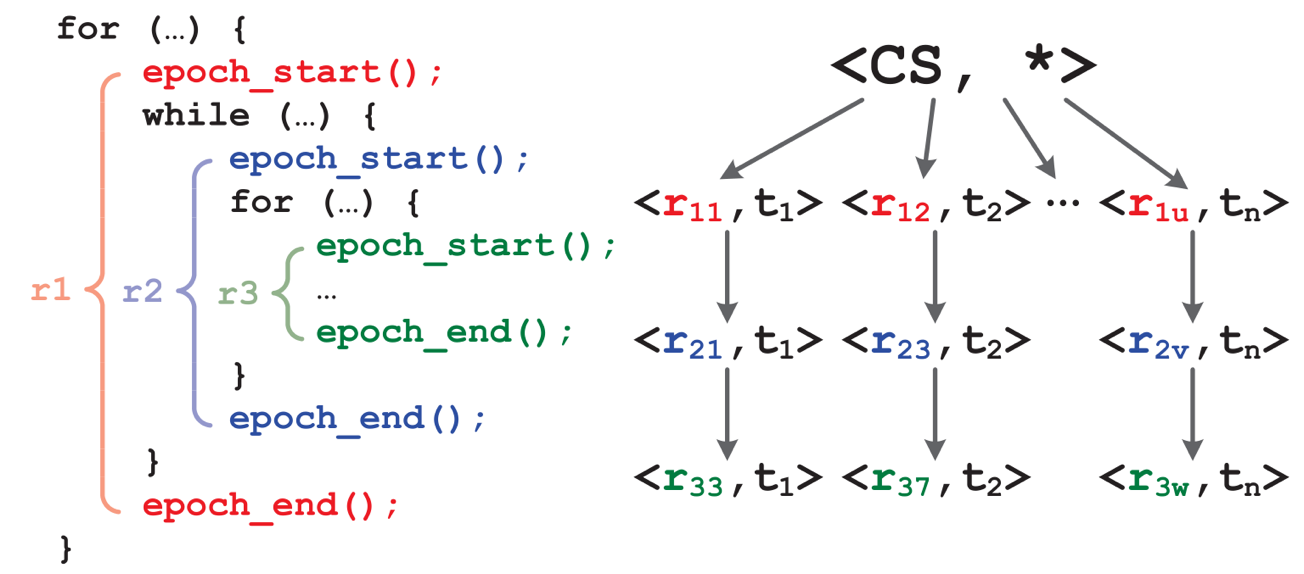
\includegraphics[width=12cm,height=7cm]{figure/epoch.png}
    \caption{
        region的一个例子:(a)一个简单的程序被多个线程执行的过程,(b)对应产生的内存域结构
    }
    \label{img2}
\end{figure}
在执行的任何时刻,可能会有多个时域,因此存在着多个内存域。基于嵌套关系,这些内存域是有一定顺序的,形成半格结构,如\ref {img2}所示,半格上的每个节点是<$r_{ij}$,$t_k$>形式的内存域,$r_{ij}$表示时期$r_i$的第$j$次执行,$t_k$表示线程。例如,区域<$r_{21}$,$t_1$>是<$r_{11}$,$t_1$>的子节点,因为在程序中,时域$r_2$是嵌套在$r_1$中的,并且执行线程相同,都是$t_1$。当被不同的线程执行时,两个时域(例如<$r_{11}$,$t_1$>和<$r_{12}$,$t_2$>)是并发的。

{\bfseries 第二个问题:如何正确并且高效地释放内存域?}

少量的对象存活时间可能比他们所处的时域存在时间长,这些存活对象必须在GC时被标识,并且迁移到安全的空间。Yak必须自动完成两项关键任务:(1)标识存活对象,(2)迁移存活对象。

对于第一项任务,Yak使用高效的算法来追踪跨内存域/空间的引用,并在运行时为每个内存域记录所有的传入引用。在内存域释放之前,Yak将这些引用作为根集合,以计算内存域中迁移对象的传递闭包。

对于第二项任务,对于每个转移对象O,Yak将O重定位到一个活内存域。为了实现这个目标,Yak标识每个传入的对O的跨内存域/跨空间引用的源内存域,并将其进行join操作,以在内存域半格上找到最小上界。例如,在图5中,对<$r_{21}$,$t_1$>和<$r_{11}$,$t_1$>进行join,返回<$r_{11}$,$t_1$>。若join了任意两个并发的区域,则返回到CS。直观地说,如果O有来自父区域和祖父区域的引用,则O应当被移动到祖父区域,如果O有来自两个不同的线程的引用,则必须被移动到CS。

在释放期间,如果其它线程访问将迁移对象的传递闭包,可能会导致不完全闭包。另外,当其他行程运行时,不能并发地移动对象,否则可能会引起数据竞争。为此,Yak使用轻量级的“stop-the-word”处理,以保证在释放时是线程安全的。当一个线程到达时域结束期,Yak暂停所有正在运行的线程,扫描它们的栈,计算释放内存域内所有潜在活对象的闭包。在其它的线程恢复前,将这些对象移动到各自的目标内存域。

Yak在Oracle的JVM OpenJDK 8 (build 25.0-b70)中实现。除了基于时域的技术,还修改了两个JIT编译器(C1和Opto),解释器,对象/堆布局,和Parallel Scavenge收集器,以管理CS。




\section{局限性}
TODO
